\chapter{LE2ML: un \textit{workbench} modulaire pour l'apprentissage machine}
\label{chap:6}

\section{Introduction}

Grâce aux chapitres précédents, il a été montré, dans un premier temps, que les \textit{wearable devices} sont de plus en plus utilisés dans le processus de reconnaissance d'activités au sein des habitats intelligents. Aussi, ces dispositifs ont également été employés dans l'objectif de répondre à plusieurs autres problématiques relatives à l'assistance des résidents de ces habitats, au sens large. Néanmoins, l'engouement croissant pour les \textit{wearable devices} a permis d'identifier plusieurs problématiques quant à leur utilisation dans ce contexte de recherche particulier. En effet, il a été évalué que la plupart des différentes architectures d'habitats intelligents qui ont été proposées n'ont pas été conçues dans une optique évolutive. Ainsi, celles-ci ne permettent pas d'y intégrer de manière rapide et efficace de nouveaux capteurs, comme les \textit{wearable devices}, ou de nouveaux composants logiciels pour réaliser le processus de reconnaissance d'activités et l'assistance aux résidents.

Pour ce travail, l'intégration des \textit{wearable devices} dans les architectures de maisons intelligentes s'est concentrée avant tout sur un aspect logiciel plutôt que matériel des différentes méthodes de reconnaissances que ces dispositifs proposent. En effet, tout comme pour la reconnaissance d'activités réalisée de manière classique, c'est-à-dire, en exploitant les capteurs et effecteurs statiques présents dans l'habitat, les différents processus proposés par les dispositifs sont, dans une vaste majorité des cas, encapsulés au sein d'un unique composant logiciel immuable. De la même manière, la réutilisation de mécanismes communs, le déploiement de ces méthodes et leur modification demeurent alors des tâches complexes à mettre en \oe{}uvre.

Malgré cela, certains travaux ont fait mention de l'emploi d'un \textit{workbench} d'apprentissage machine afin de traiter les données produites par les \textit{wearable devices} et effectuer la reconnaissance d'activité \citep{Chapron2018}. D'un point de vue académique, ces outils ne sont pas nouveaux et ils permettent un prototypage rapide, la visualisation des données ainsi qu'une meilleure reproductibilité des méthodes expérimentales et une meilleure réutilisation des composants logiciels \citep{Holmes1994,Langlois2008}. À titre d'exemple, l'outil le plus connu et le plus répandu dans la littérature est \acs{WEKA}. Il s'agit d'un \textit{workbench} open source développé en Java qui supporte un grand nombre d'algorithmes d'apprentissage machine supervisés et non supervisés \citep{Witten2016}. Celui-ci a été utilisé en tant que librairie dans la méthode de reconnaissance des types de sols présentée au chapitre \ref{chap:4}. Néanmoins, bien que ce \textit{workbench} offre un large éventail d'options, son utilisation reste relativement gourmande en termes d'utilisation des ressources de calcul et de mémoire. De plus, les fonctionnalités offertes par cet outil demeurent particulièrement contraignantes à étendre et de par sa conception, il n'est pas particulièrement adapté pour être utilisé dans l'architecture d'habitats intelligents distribuée qui a été introduite dans le chapitre précédent. Par ailleurs, avec la tendance qui entoure actuellement l'intelligence artificielle, ce type d'outil devient de plus en plus populaire depuis que des fournisseurs de \textit{cloud} publics, tels qu'\textit{Amazon AWS}, \textit{Google Cloud Plateform} et \textit{Microsoft Azure} ont introduit des versions grand public de ces applications. Comme elles font partie de la vaste liste de services payants proposés par chaque fournisseur, les \textit{workbench} d'apprentissage machine peuvent bénéficier de l'évolutivité qu'offre le \textit{cloud}. Cependant, comme ils sont considérés comme des services d'usage général, les mécanismes internes des techniques d'apprentissage machine ont été complètement occultés afin de les rendre accessibles à tous.

Ainsi, ce dernier travail présente \acs{LE2ML} (\acl{LE2ML}), un nouveau type de \textit{workbench} pour l'apprentissage machine qui repose sur l'utilisation de microservices. De la même manière que pour l'implémentation de l'architecture proposée, cette conception logicielle a été choisie, car la technologie des microservices permet une meilleure évolutivité, des déploiements plus sûrs et plus rapides ainsi qu'une meilleure isolation des pannes \citep{Dragoni2017}. Cependant, l'avantage principal d'une telle conception concerne l'aspect modulaire que permettent les microservices. Ainsi, ce \textit{workbench} demeure un outil agnostique tant en termes de langages de programmation que de plateformes supportées qui peut être déployé dans n'importe quel environnement, et ce, sans aucune contrainte complexe.

La suite de ce chapitre comporte une première section qui propose un état de l'art en matière de \textit{workbench} pour l'apprentissage machine, car ceux-ci ont joué, depuis plusieurs années, un rôle important dans différents champs de recherche. Ensuite, la section suivante introduit \acs{LE2ML}, le \textit{workbench} proposé et une expérimentation pour évaluer son fonctionnement et valider les résultats attendus est décrite dans une troisième section. Finalement, dans une dernière partie, ce chapitre dresse une conclusion quant à ce dernier travail.

\section{État de l'art}

\subsection{WEKA}

\begin{figure}[H]
	\centering
	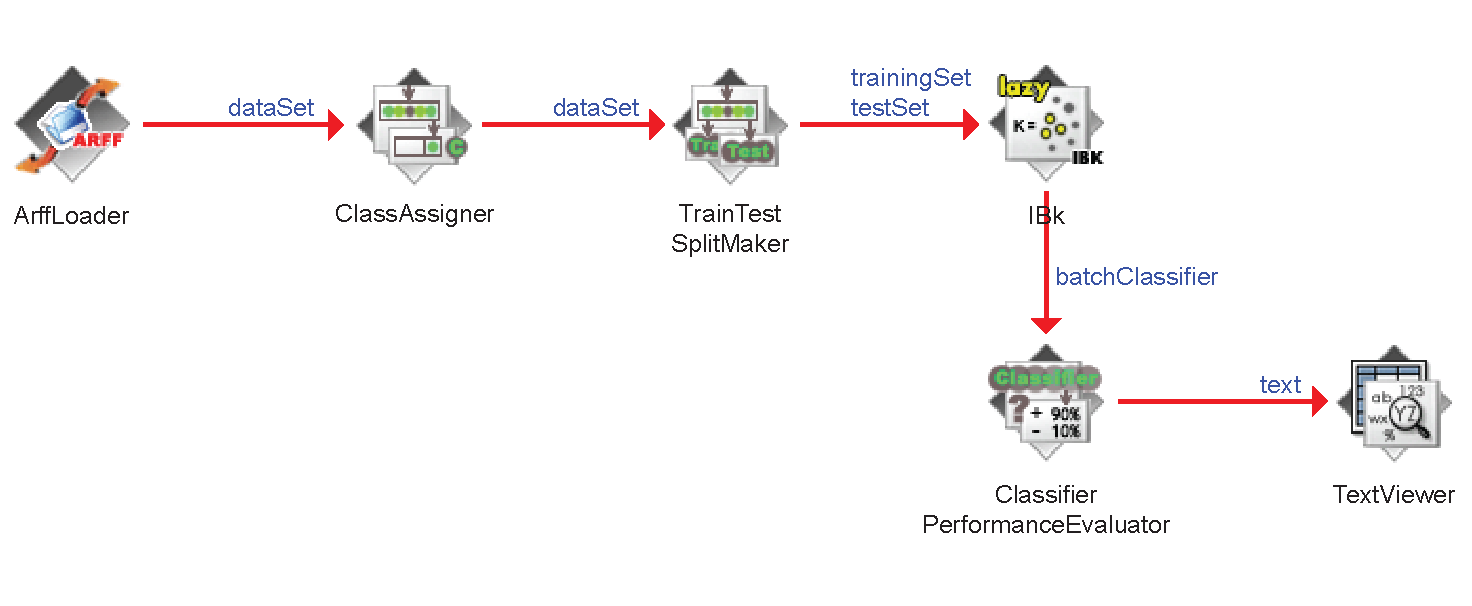
\includegraphics[width=.9\linewidth]{chapter6/weka.pdf}
        \caption{caption}
	\label{fig:weka}
\end{figure}

\subsection{RapidMiner}

\begin{figure}[H]
	\centering
	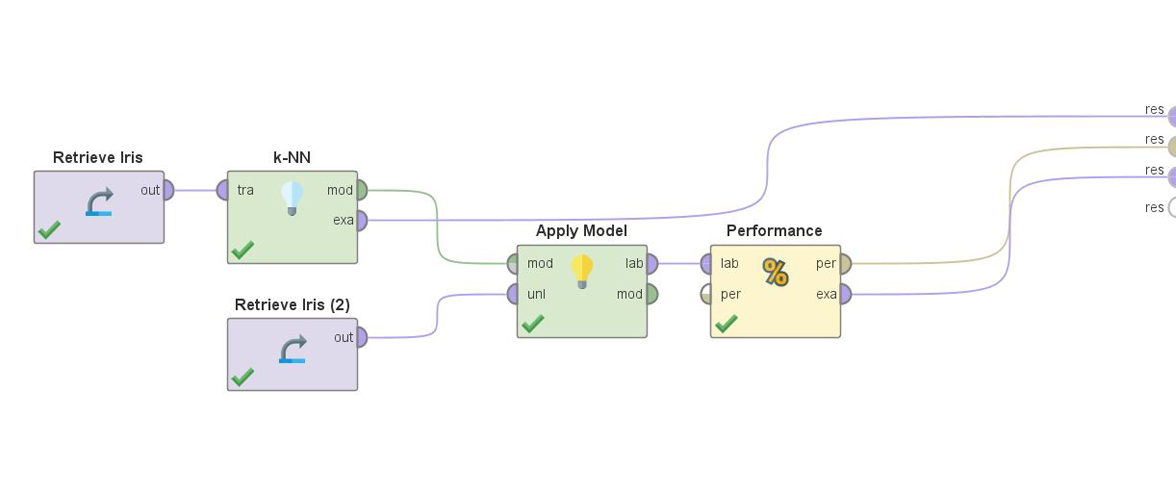
\includegraphics[width=.9\linewidth]{chapter6/rapid_miner.jpg}
        \caption{caption}
	\label{fig:rapid_miner}
\end{figure}

\subsection{Orange}

\begin{figure}[H]
	\centering
	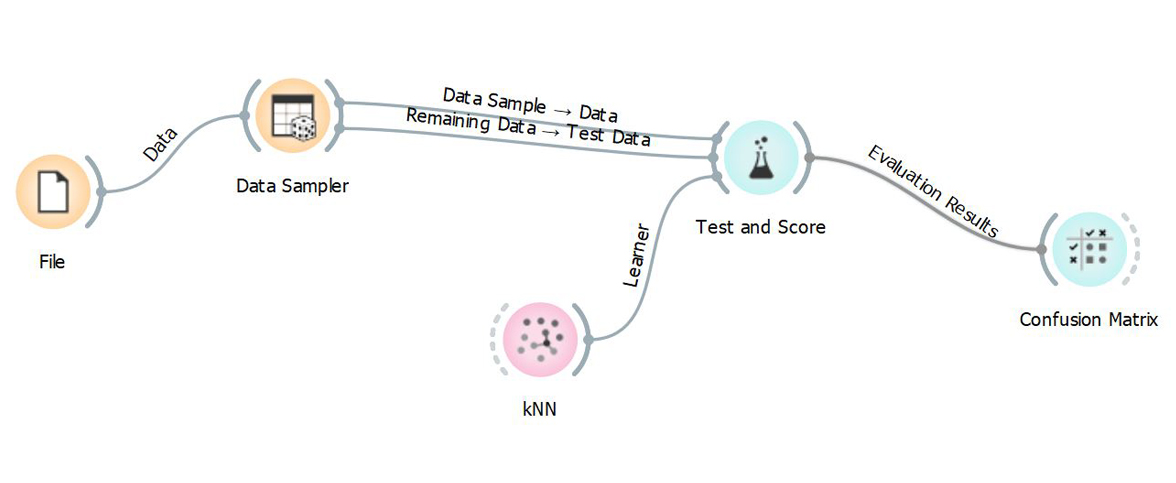
\includegraphics[width=.9\linewidth]{chapter6/orange.jpg}
        \caption{caption}
	\label{fig:orange}
\end{figure}

\section{Solution proposée}

\begin{figure}[H]
	\centering
	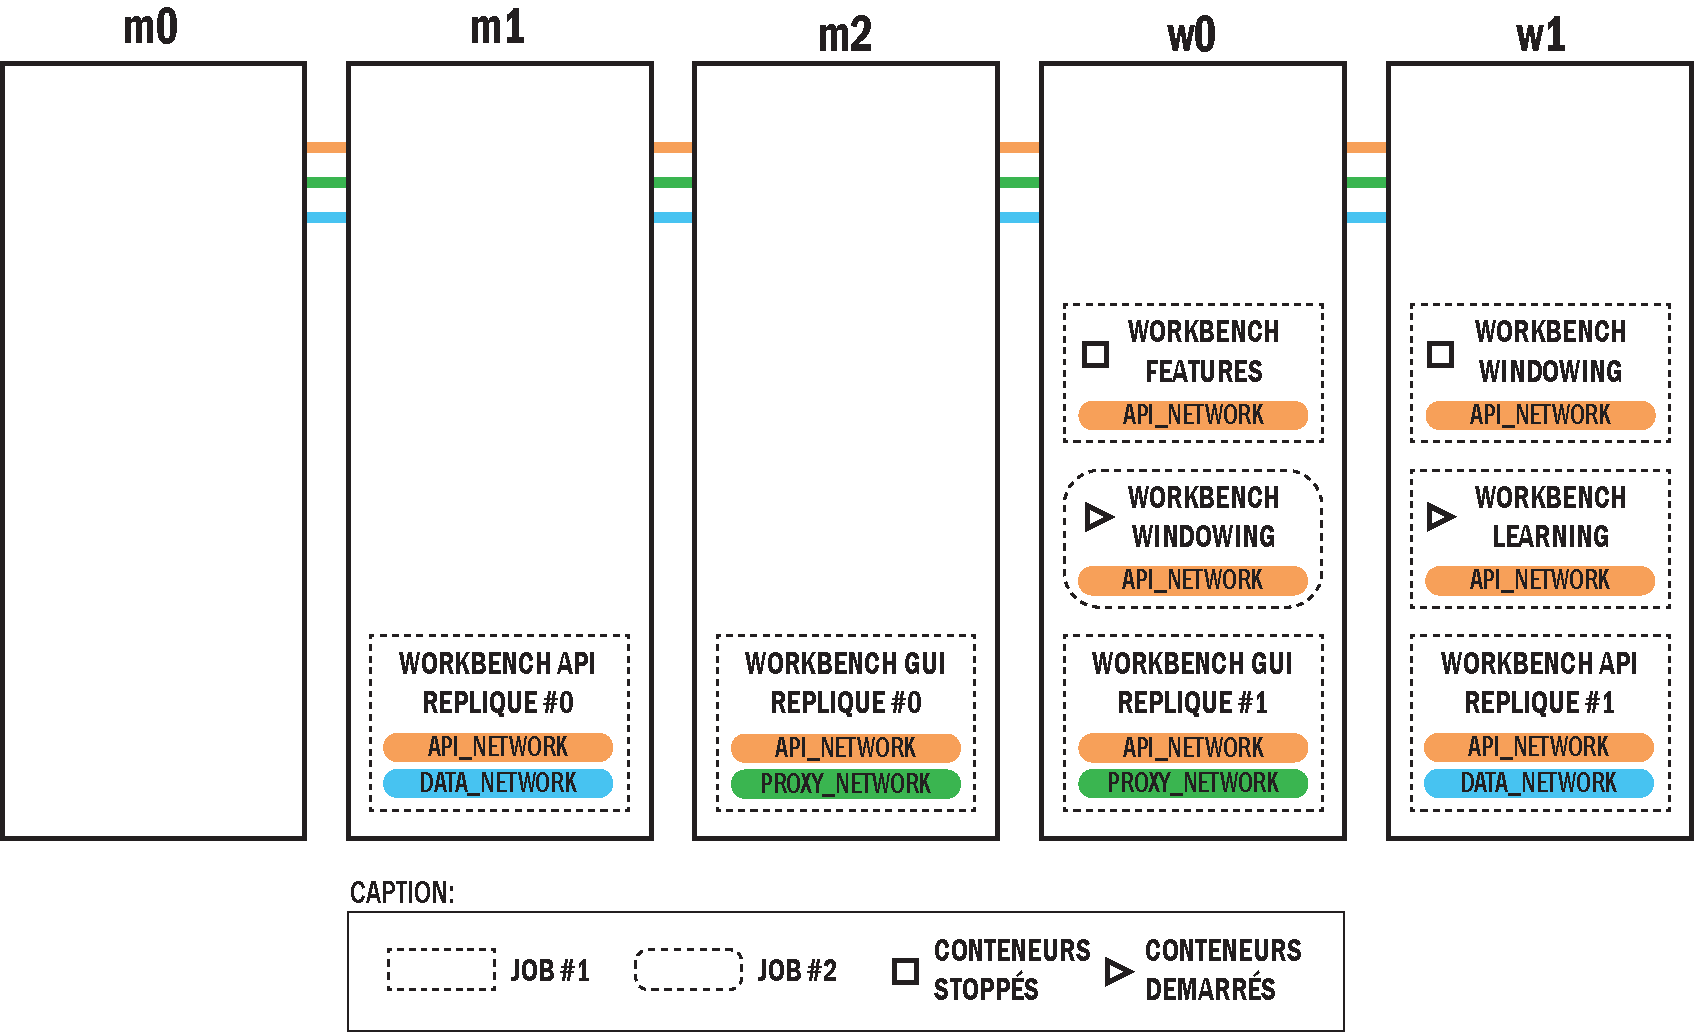
\includegraphics[width=.9\linewidth]{chapter6/containers_workbench.pdf}
        \caption{caption}
	\label{fig:containers_workbench}
\end{figure}

\subsection{API REST}

\begin{figure}[H]
	\centering
	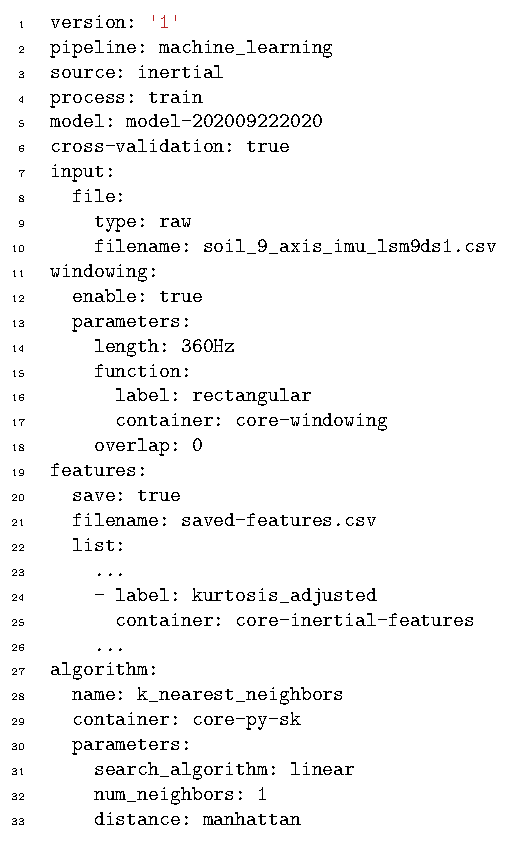
\includegraphics[width=.5\linewidth,keepaspectratio]{chapter6/pipeline_conf.pdf}
        \caption{caption}
	\label{fig:pipeline_conf}
\end{figure}

\subsection{Application Web}

\begin{figure}[H]
	\centering
	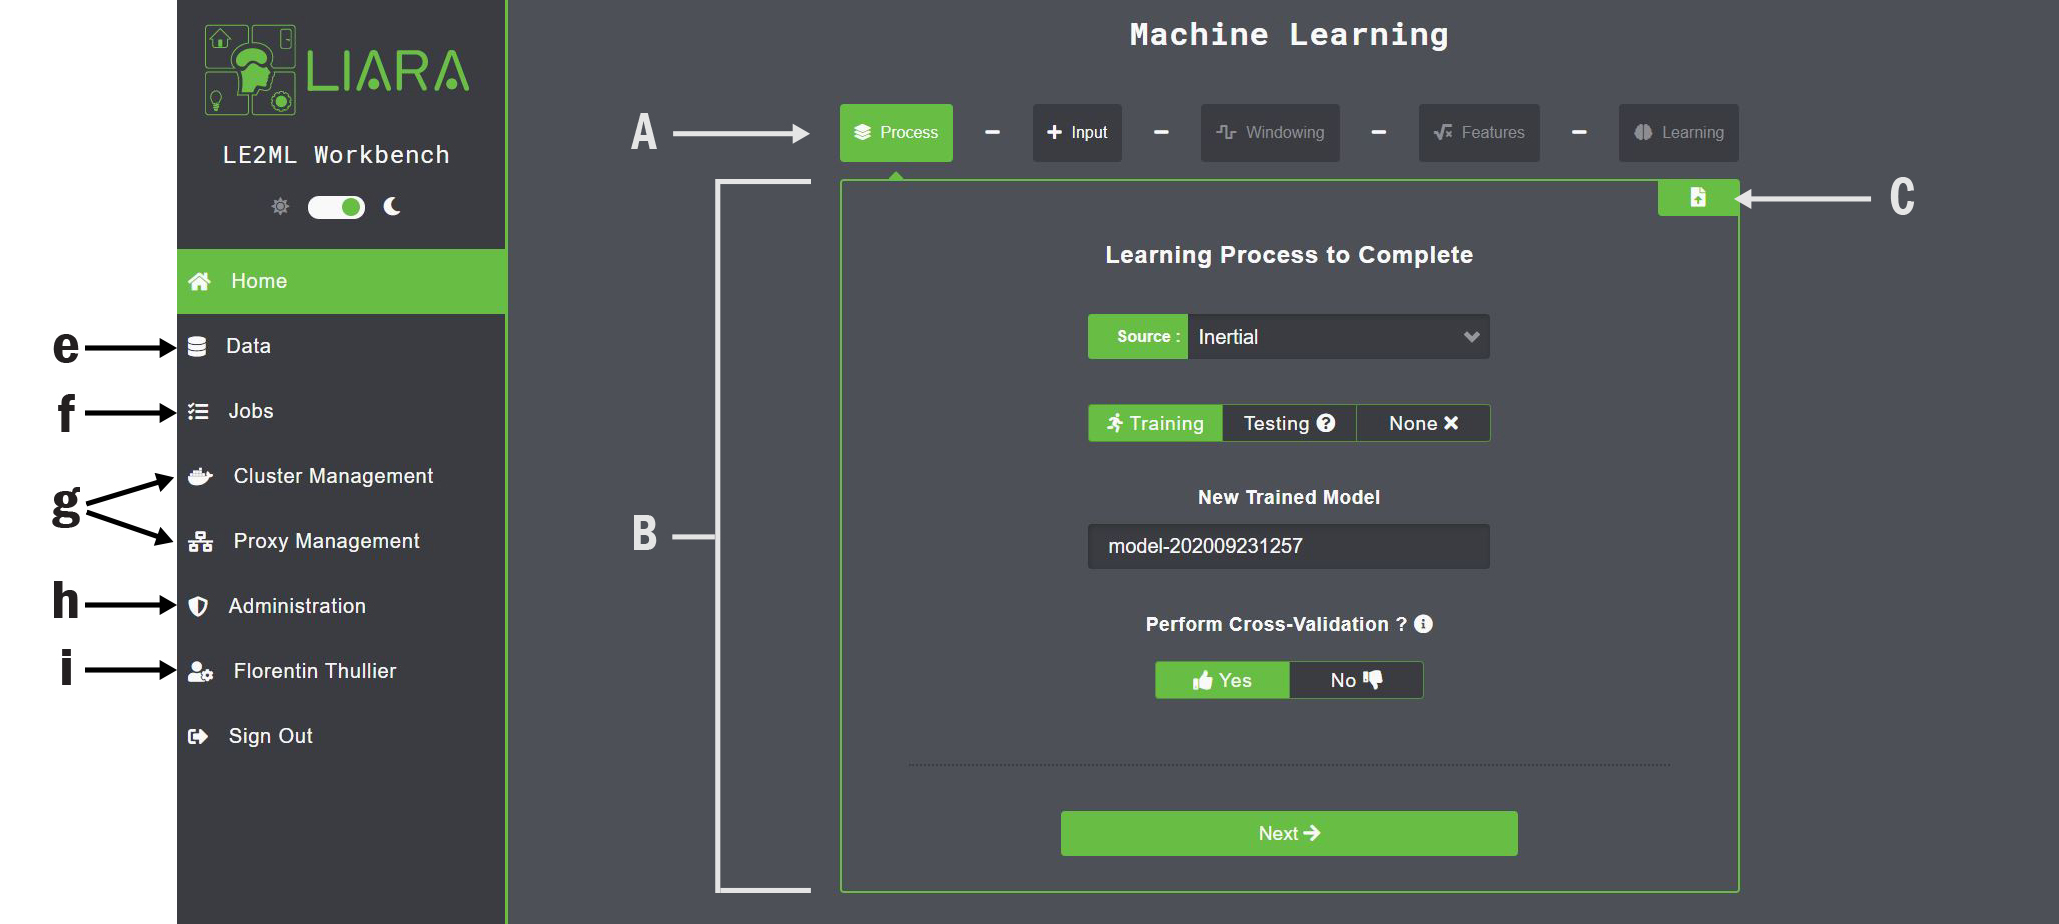
\includegraphics[angle=90,origin=c,height=\textwidth,keepaspectratio]{chapter6/le2ml_gui.jpg}
        \caption{caption}
	\label{fig:le2ml_gui}
\end{figure}

\subsection{Modules proposés}

\subsubsection{Fenêtrage}

\subsubsection{Extraction de caractéristiques}

\subsubsection{Apprentissage machine}

\section{Expérimentations \& Résultats}

\begin{table}[H]
    \centering
    \caption{caption.}
    \label{tab:previous_results}
    \begin{tabular}{@{}rccc@{}}
      \toprule
      \multicolumn{1}{l}{}              & \textit{Justesse}  &  $F\mbox{-} mesure$  & \textit{Kappa de Cohen}  \\ \midrule
      \textbf{$k$-NN}                   & 0.93               & 0.93                 & 0.89                     \\
      \textbf{\textit{Random Forest}}   & 0.92               & 0.92                 & 0.88                     \\ \bottomrule
    \end{tabular}
\end{table}

\begin{table}[H]
    \centering
    \caption{caption.}
    \label{tab:l2ml_results}
    \begin{tabular}{@{}rccc@{}}
      \toprule
      \multicolumn{1}{l}{}              & \textit{Justesse}  &  $F\mbox{-} mesure$  & \textit{Kappa de Cohen}  \\ \midrule
      \textbf{$k$-NN}                   & 0.91               & 0.91                 & 0.86                     \\
      \textbf{\textit{Random Forest}}   & 0.92               & 0.92                 & 0.88                     \\ \bottomrule
    \end{tabular}
\end{table}

\section{Conclusion}
